\subsubsection{\stid{3.14} ALExa}


\paragraph{Overview}

The ALExa project ({\sl Accelerated Libraries for Exascale}) focuses on
preparing the ArborX, DTK, Tasmanian, and ForTrilinos libraries for exascale
platforms and integrating these libraries into ECP applications.
These libraries deliver capabilities identified as needs of ECP applications:
%
(1) the ability the perform performance portable spatial searches between
arbitrary sets of distributed geometric objects (ArborX);
%
(2) the ability to transfer computed
solutions between grids with differing layouts on parallel accelerated
architectures, enabling multiphysics projects to seamlessly combine results
from different computational grids to perform their required simulations
(DTK); and
%
(3) the ability to construct fast and memory efficient surrogates to
large-scale engineering models with multiple inputs and many outputs,
enabling uncertainty quantification (both forward and inverse) as well as
optimization and efficient multi-physics simulations in projects such as
ExaStar (Tasmanian); and
%
(4) the ability to automatically interface Fortran-based codes to existing
large and complex C/C++ solftware libraries, such as Trilinos advanced solvers
that can utilize next-generation platforms.


These capabilities are being developed through ongoing interactions with our
ECP application project collaborators to ensure they will satisfy requirements
of these customers.  The libraries in turn take advantage of other ECP/SW
capabilities currently in development, including Trilinos,
Kokkos, and SLATE.  The final outcome of the ECP project will be a set of
libraries deployed to facilities and also made broadly available as part of
the xSDK4ECP project.


{\bf ArborX}

{\it Purpose:} ArborX is an open-source library designed to provide
performance portable algorithms for geometric search.

{\it Significance:} General geometric search capabilities are needed in a wide
variety of applications, including the generation of neighbor lists in
particle-based applications (e.g., molecular dynamics or general N-body
dynamics simulations), density-based clustering analysis (e.g., halo finding
or DBSCAN in cosmology) and mesh-mesh interactions such as contact in
computational mechanics and solution transfer in multiphysics simulations.

{\it Performance portable search capabilities:} Shared memory and GPU
implementations of spatial tree construction; shared memory and GPU
implementations of various spatial tree queries; MPI front-end for
coordinating distributed spatial searches between sets of geometric objects
with different decompositions; communication plan generation based on spatial
search results; density-based clustering algorithms (DBSCAN).

{\it URL:} https://github.com/arborx/ArborX

{\bf DTK} (Data Transfer Kit)

{\it Purpose:} Transfers computed solutions between grids with differing
layouts on parallel accelerated architectures.

{\it Significance:} Coupled applications frequently have different grids with
different parallel distributions; DTK is able to transfer solution values
between these grids efficiently and accurately.

{\it Mesh and mesh-free interpolation capabilities:} multivariate data
interpolation between point clouds and grids; compactly supported radial basis
functions; nearest-neighbor and moving least square implementations; support
for standard finite-element shape functions and user-defined interpolants;
common applications include conjugate heat transfer, fluid structure
interaction, and mesh deformation.

{\it URL:} https://github.com/ORNL-CEES/DataTransferKit


{\bf Tasmanian} (Toolkit for Adaptive Stochastic Modeling and Non-Intrusive
Approximation)

{\it Purpose:} Constructs efficient surrogate models for high-dimensional
problems and performs parameter calibration and optimization geared towards
applications in uncertainty quantification (UQ).

{\it Significance:} UQ pertains to the statistical properties of the output
from a complex model with respect to variability in multiple model inputs;
large number of simulations are required to compute reliable statistics which
is prohibitive when dealing with computationally expensive engineering
models. A surrogate model is constructed from a moderate set of simulations
using carefully chosen input values; analysis can then be performed on the
efficient surrogate.

{\it Sparse grids capabilities:} surrogate modeling and design of experiments
(adaptive multi-dimensional interpolation); reduced (lossy) representation of
tabulated scientific data; high dimensional numerical quadrature; data mining
and manifold learning.

{\it DiffeRential Evolution Adaptive Metropolis (DREAM) capabilities:}
Bayesian inference; parameter estimation/calibration; model validation.
global optimization and optimization under uncertainty.

{\it URL:} http://tasmanian.ornl.gov


{\bf ForTrilinos} (Fortran Trilinos)

{\it Purpose:}
ForTrilinos provides a seamless pathway for large and complex Fortran-based
codes to access Trilinos without C/C++ interface code. This access includes
Fortran versions of Kokkos abstractions for code execution and data management.
To provide this functionality, this project developed a Fortran-targeted
extension to the SWIG (Simplified Wrapper and Interface Generator) tool.
Applied to Trilinos, it generates object-oriented Fortran 2003 interface code
that closely mirrors the Trilinos C++ API.

{\it Significance:}
The Exascale Computing Project (ECP) requires the successful transformation and
porting of many Fortran application codes in preparation for ECP platforms. A
significant number of these codes rely upon the scalable solution of linear and
nonlinear equations. The Trilinos Project contains a large and growing
collection of solver capabilities that can utilize next-generation platforms, in
particular scalable multicore, manycore, accelerator and heterogeneous systems.
Since Trilinos is written primarily in C++, its capabilities are not available
to other programming languages. ForTrilinos bridges the gap between the
needs of Fortran app developers and the capabilities of Trilinos. Furthermore,
the technology used to generate the Fortran--C++ bindings in ForTrilinos is
capable of exposing any number of C++ libraries to Fortran exascale app
developers.


{\it SWIG capabilities:}
ForTrilinos provides an inversion of control functionality that enables custom
extensions of the Trilinos solvers implemented in downstream Fortran apps.
Although this capability is not yet comprehensive, the goal of this project is
to provide functional and extensible access Trilinos on next-generation
computing systems. Several examples of ForTrilinos are being demonstrated within
Fortran-based ECP codes to help them meet simulation goals and illustrate the
technology to other Fortran-based ECP codes. Additionally, the SWIG technology
underpinning ForTrilinos is being applied to other C++-based ECP ST subprojects
to expose their capabilities to Fortran apps.

{\it URL:} https://github.com/trilinos/ForTrilinos

\paragraph{Key Challenges}

\indent

{\bf ArborX:} Search procedures to locate neighboring points, mesh cells, or
other geometric objects require tree search methods difficult to optimize on
modern accelerated architectures due to vector lane or thread divergence. A
flexible interface for calling user kernels on a positive match as well as
modifying traversal algorithms in a task-specific manner are crucial to
achieving the best performance.

{\bf DTK:} General data transfer between grids of unrelated applications
requires many-to-many communication which is increasingly challenging as
communication to computation ratios are decreasing on successive HPC systems.
Maintaining high accuracy for the transfer requires careful attention to the
mathematical properties of the interpolation methods and is highly
application-specific.

{\bf Tasmanian:} Extracting statistical information from a Tasmanian surrogate
(or using the surrogate in a multi-physics simulation) requires the collection
of a large number of samples, which is not feasible without GPU acceleration.
The GPU accelerated surrogate evaluations require both custom kernels
corresponding to the different types of basis functions as well as both
sparse and dense linear algebra methods (BLAS level 2 and 3).
Porting the capabilities and optimizing the performance across different
divergent architectures is challenging.

{\bf ForTrilinos:}
Developing the interfaces to the C++ libraries that provide access to
cutting-edge research, such as Trilinos,  is of significant benefit to Fortran
community. However, such interfaces must be well documented, sustainable and
extensible, which would require significant amount of resources and investment.
This is further complicated by the requirements to support heterogeneous
platforms (e.g., GPUs) and inversion-of-control functionality. The manual
approach to such interfaces has been shown to be unsustainable as it requires
interface developers to have in-depth expertise in  multiple languages and the
peculiarities in their interaction on top of the time commitment to update the
interfaces with changes in the library.

ForTrilinos addresses both the issue of reducing interface generation cost
through investment in tool configuration and usage to make the process as
automatic as possible, and the issue of providing the full-featured interface to
Trilinos library, including access to manycore, accelerator and heterogeneous
solver capabilities in Trilinos.


\paragraph{Solution Strategy}

\nobreak


\indent

{\bf ArborX:} ArborX builds on a MPI+Kokkos programming model to deploy to all
DOE HPC architectures. Extensive performance engineering has yielded
implementations that are both as performant in serial as state-of-the-art
libraries while also expanding on the capability provided by other libraries by
demonstrating thread scalability on both GPU and multi-core CPU architectures.
Working with both synthetic as well as real data from applications (e.g., HACC)
ensures wide performance testing coverage.

{\bf DTK:} State-of-the-art, mathematically rigorous methods are used in DTK
to preserve accuracy of interpolated solutions.  Algorithms are implemented in
a C++ code base with extensive unit testing on multiple platforms.  Trilinos
packages are used to support interpolation methods.  Kokkos is used to achieve
performance portability across accelerated platforms.

{\bf Tasmanian:} The C++ kernels within Tasmanian (currently tuned for Nvidia
Volta architecture) are templated exposing numerous performance tweaks and
tuning parameters that can be adjusted to perform well on a corresponding AMD
system.
The kernels also need to be ported to DPC++/SYCL to allow for the utilization
of Intel GPUs. Tasmanian requires a general GPU-BLAS interface that can
utilize any of the accelerated backends, e.g., cuBlas, rocBlas, MKL and MAGMA.

{\bf ForTrilinos:}
ForTrilinos defines several SWIG-Fortran modules that generate Fortran-2003
interfaces to C++ Trilinos solver classes. ForTrilinos provides a
``high-level'' interface for applications to access nonlinear and eigenvalue
solvers in addition to low-level Trilinos classes.

%----------------------------------------

\paragraph{Recent Progress}

\indent

{\bf ArborX:} Collaboration with partner application ExaSky (WBS 2.2.3.02)
resulted in significant advances for the in-situ density-based clustering
algorithm (halo finding) using Nvidia GPUs.

\begin{figure}[htb]
        \centering 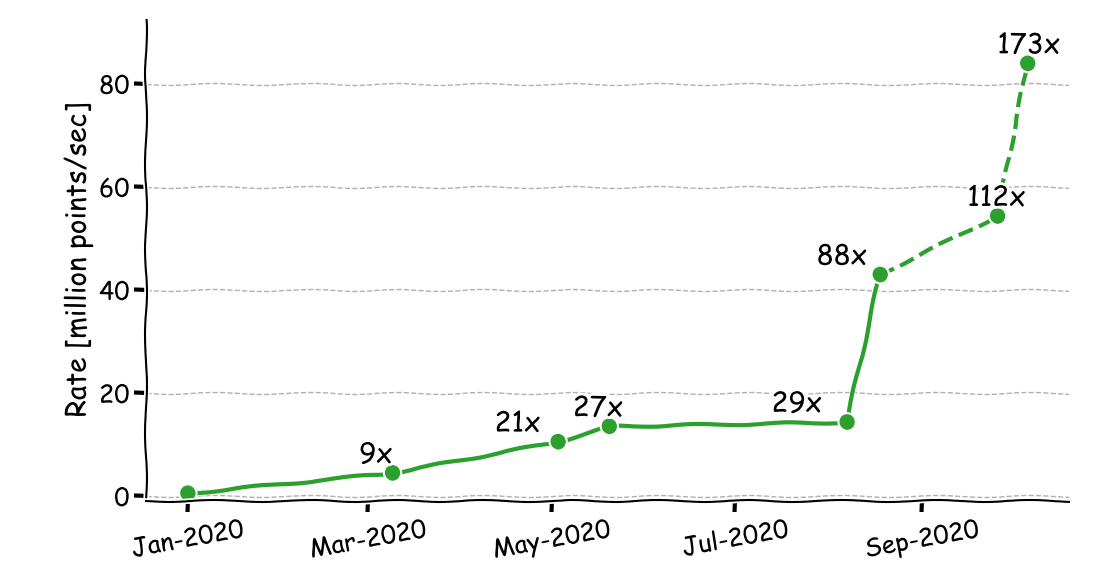
\includegraphics[width=4.0in]{projects/2.3.3-MathLibs/2.3.3.14-ALExa-ForTrilinos/arborx_hacc_progress.png} \caption{\label{fig:arborx-hacc}
        ArborX progress on halo finding algorithm on Nvidia Volta. The baseline
        is a serial implementation of CosmoTools. Numbers indicate speedup
        compared to the baseline. The solid lines show improvements that were
        already merged. Dashed lines show improvements that are in active
        development. }
\end{figure}

{\bf DTK:} DTK's build system has been rewritten. DTK now depends on Trilinos
instead of being built as an external package. DTK is now a separate package in
spack. In the future this will allow a decoupling between Trilinos version and
DTK version. A new spline interpolation method has been added.

{\bf Tasmanian:} Work with partner application ExaStar (2.2.3.01) created a
reduced representation of neutrino opacities used by the Thornado simulation
software. The classical representation uses dense tables that do not fit in
GPU memory and lead to unnecessary and expensive data movement for each time-step.
The reduced representation by Tasmanian preserved the accuracy of the simulations
and dramatically reduces the memory footprint by removing redundancies
and exploiting smoothness in the data.

\begin{figure}[htb]
        \centering
        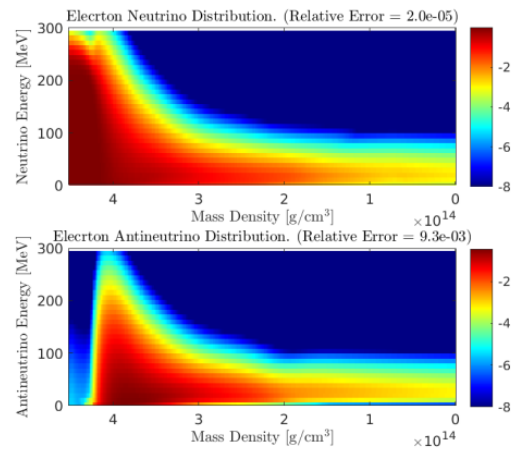
\includegraphics[width=2.5in]{projects/2.3.3-MathLibs/2.3.3.14-ALExa-ForTrilinos/tasmanian_exastar}
\caption{\label{fig:tasmanian-exastar}
		The resulting neutrino and antineutrino distributions in a deleptonization
		wave simulation using sparse grid opacities, which require only 6\% of
		the memory used in the dense approach, with relative $L^2$ error less than 1\%.}
\end{figure}

{\bf ForTrilinos:}
As with DTK, ForTrilinos now has an independent build system with Trilinos as a
dependency. This improves robustness of the build and makes ForTrilinos
available to app developers even if a system installation of Trilinos does not
enable Fortran. ForTrilinos is now independently available through the Spack
package manager. New ST libraries including Tasmanian have been wrapped with the
SWIG-Fortran utility.

%----------------------------------------

\paragraph{Next Steps}

\indent

{\bf ArborX:} Incorporate non axis-aligned bounding volumes to accommodate
stretched inclined geometries such as those coming from wind turbine
simulations from ExaWind (WBS 2.2.2.01). Further improve performance of
density-based algorithms.

{\bf DTK:} Continue performance engineering campaign and deploy in a variety of
applications.

{\bf Tasmanian:} Port the surrogate evaluation kernels to AMD and Intel
GPUs and optimize the performance on the next generation architectures
(including next generation Nvidia GPUs).

{\bf ForTrilinos:} Extend ForTrilinos native Fortran interface documentation and
prioritize Fortran app customer needs. Integrate SWIG into ECP ST projects that
desire Fortran interfaces.

%----------------------------------------
